\documentclass[11pt]{article}
\ifdefined\anonymous
\usepackage[review]{acl}
\else
\usepackage{acl}
\fi
\usepackage{times}
\usepackage{latexsym}
\usepackage[T1]{fontenc}
\usepackage[utf8]{inputenc}
\usepackage{microtype}
\usepackage{graphicx}
\usepackage{booktabs}
\usepackage{amsmath,amssymb,amsthm}
\usepackage{listings}
\newtheorem{proposition}{Proposition}
\newcommand{\wire}{\mathcal{W}}
\newcommand{\val}{\mathcal{V}}
\title{Before the Validator: Numeric Wire Fidelity in LLM Tool Pipelines}
\author{Shivam Gupta \\
 Independent Researcher \\
 \texttt{shivam1720406@gmail.com}}
\begin{document}
\maketitle
\begin{abstract}
Schema compliance and value preservation are different properties of language-model tool interfaces. An argument can satisfy its numeric schema, pass an SDK parser and downstream validator, and nevertheless select a different record. We study this boundary through an exact rational oracle, a census of 9,558 public schemas, and execution of a pinned Model Context Protocol (MCP) implementation. After excluding two files with duplicate keys, we extract 34,357 local numeric projections and test 8,207 distinct schema--value pairs. Native JavaScript transport changes 2,600 values; 2,349 changes pass an Ajv validator. A post-parse safe-integer check still admits 479 changed values. In a local MCP record-lookup experiment, 25 of 54 constructed integer requests select the wrong fixture record. A pre-parse guard prevents these changes by rejecting them, while an explicit string identifier contract completes all 54 lookups correctly. Existing lossless JSON serialization preserves every stress-test value. These findings support adding transport fidelity to tool-system evaluation, without claiming a new numeric representation, a model failure rate, or production deployment evidence.
\end{abstract}

\section{Introduction}
A language model emits the integer identifier \texttt{9007199254740993}. The tool schema allows integers, the JSON is well formed, and a downstream validator accepts the parsed argument. A JavaScript middleware layer has already converted the identifier to \texttt{9007199254740992}. If both identifiers name records, the tool can complete successfully against the wrong record. Neither the model's original bytes nor the intended identifier need appear in an ordinary post-parse execution log.

This is an established interoperability hazard in a consequential interface. JSON and I-JSON document numeric precision limits and recommend string representations when greater precision is required \citep{bray2017,bray2015}. Cross-language parser discrepancies have also been systematically studied \citep{moeller2024}. The question here is therefore not whether floating-point numbers can lose precision. It is whether the evaluation boundary commonly used for structured outputs distinguishes a valid emitted value from a value changed by the surrounding tool infrastructure.

Structured generation evaluates constraint compliance, coverage, speed, and task quality \citep{geng2025,dong2025,lu-etal-2025-learning}. MCP exposes tool input schemas and structured arguments \citep{mcp2025}. These interfaces create two numeric transport surfaces: the argument and the schema specifying its constraints. Checking only the argument can miss a schema whose bound or numeric constant has already changed. Conversely, preserving both wire representations does not make floating-point validator arithmetic exact.

We investigate three questions. RQ1: Which numeric values and schema literals change under the tested transport? RQ2: Which changes survive downstream schema validation or a safe-integer check? RQ3: What availability and runtime trade-offs arise from established lossless transport, an explicit string identifier contract, and a pre-parse fidelity guard?

Our contribution is an empirical audit and executable evaluation protocol. It combines source-literal measurements, schema-conditioned stress cases, and a live local MCP handler, with separate denominators for each. The guard is a reference implementation of a value-preservation check, not a claim to invent safe parsing. The results do not establish the prevalence of these failures in model generations or deployed products.

\begin{figure*}[t]
\centering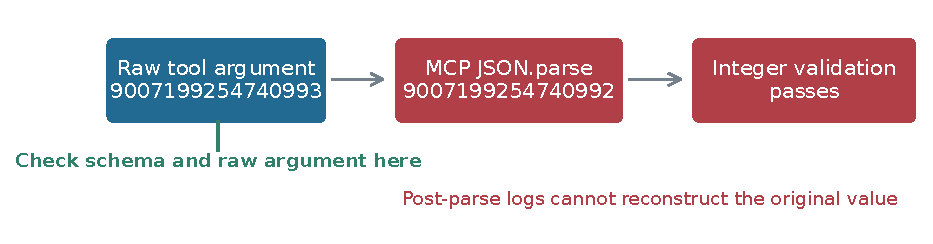
\includegraphics[width=\textwidth]{figures/boundary.pdf}
\caption{A correct emitted integer can become a different valid integer before a tool handler runs. Fidelity evidence must retain the raw argument and the relevant schema before their first lossy parse. The figure depicts the local reproduction, not an observed customer incident.}
\label{fig:boundary}
\end{figure*}

\section{Related Work and Contribution Boundary}
\paragraph{Parser interoperability.}
\citet{moeller2024} differentially test 22 JSON parsers and analyze numeric, string, and object discrepancies. Their work establishes the general problem and its security relevance. I-JSON explicitly warns about integers outside the interoperable range \citep{bray2015}; JSON canonicalization builds on an agreed representation domain \citep{rundgren2020}. We add a schema-conditioned audit of an LLM tool transport, separating value drift from validation success. We do not claim that parser disagreement is new or that the tested SDK violates JSON's permitted implementation limits.

\paragraph{Structured-output evaluation.}
JSONSchemaBench evaluates generation efficiency, constraint coverage, and output quality using real-world schemas \citep{geng2025}. XGrammar provides efficient structured generation \citep{dong2025}, while Schema Reinforcement Learning trains models toward schema adherence \citep{lu-etal-2025-learning}. Function-calling robustness research examines broader weaknesses in agent evaluation \citep{rabinovich2025}. Our experiment holds the emitted bytes fixed and studies subsequent infrastructure. It neither benchmarks a decoder nor attributes transport-induced changes to a model.

\paragraph{Schema analysis and remedies.}
Witness generation and subschema checking address schema satisfiability and compatibility \citep{attouche2022,habib2021}. Bowtie compares validator behavior across implementations \citep{berman2023}. We use local numeric projections rather than a complete schema witness generator. The existing \texttt{lossless-json} library preserves numeric tokens and provides safety checks \citep{deJong2026}; it is a central baseline. Our contribution is the combined measurement and failure localization, rather than a replacement for these techniques.

\section{An Explicit Fidelity Contract}
\subsection{Wire values and validation}
Let $b$ be a JSON number token and $\val(b)\in\mathbb{Q}$ its exact mathematical decimal value. Let
\begin{equation}
 \wire(b)=\operatorname{stringify}(\operatorname{parse}(b))
\end{equation}
be a specified runtime's parse--serialize transformation. Numeric wire fidelity holds when $\wire(b)$ is numeric and
\begin{equation}\label{eq:fidelity}
 F(b) = [\val(b)=\val(\wire(b))].
\end{equation}
For trees, we compare numbers recursively, preserving object keys, array order, strings, booleans, and nulls. Duplicate keys are outside this contract. We identify $-0$ with $0$ and identify equivalent decimal spellings; the property is not byte preservation. It is also not exact binary representation: \texttt{0.1} can satisfy Eq.~\ref{eq:fidelity} even though its binary64 representation is inexact.

For a numeric schema $S$ and token $b$, define $A(S,b)$ as exact reference acceptance. The stress suite retains only $A(S,b)=1$. A \emph{hidden change} occurs when $F(b)=0$ but the tested native validator accepts the parsed argument against the parsed schema. This operational definition does not assume that the validator's acceptance agrees with an exact reference after transport.

Schema fidelity is checked separately: numeric literals in the serialized schema must preserve their mathematical values. A changed \texttt{default} or \texttt{example} affects documentation or initialization; a changed bound can affect accepted values. We report these categories separately and do not treat every numeric annotation as an assertion.

\subsection{Why post-parse evidence is insufficient}
\begin{proposition}\label{prop:collision}
If two distinct numeric values have the same parsed native value, a checker that receives only that parsed value cannot both accept every faithful source token and reject every unfaithful source token.
\end{proposition}
\begin{proof}
Let $b_0$ and $b_1$ parse to the same value, with $F(b_0)=1$ and $F(b_1)=0$. The checker receives identical input for both tokens and must return the same decision. Accepting $b_0$ therefore accepts $b_1$, while rejecting $b_1$ rejects $b_0$. For JavaScript, \texttt{9007199254740992} and \texttt{9007199254740993} instantiate the argument.
\end{proof}
This elementary collision argument locates necessary evidence. Revalidating the already parsed value, signing that value, or logging it more extensively cannot reconstruct the discarded token. Retaining original bytes or a lossless representation can.

A schema collision creates a related problem. Consider the schema with integer constant \texttt{9007199254740993} and argument \texttt{9007199254740992}. Exact validation rejects the argument. Native parsing maps the constant to the argument, and Ajv accepts. The argument itself is wire-faithful, so an argument-only guard cannot detect the changed contract. Schema capture must precede schema parsing as well.

\subsection{Pre-parse guard and scope of its guarantee}
The reference guard uses Node's JSON reviver source context to compare each original numeric token with the native serializer's output. A decimal token is represented as a signed integer coefficient and a base-ten exponent; trailing zeros are removed using integer arithmetic. Zero receives one canonical representation. Non-finite parsed numbers and unequal normalized pairs cause rejection.

For a fixed native serializer, this accepts exactly the numeric tokens satisfying Eq.~\ref{eq:fidelity}: coefficient--exponent normalization decides equality of finite decimal rational numbers. Applied recursively, the same check preserves numeric wire values in the assumed tree domain. Applying it to both schema and argument prevents their numeric wire drift. It does \emph{not} prove equivalence of validator arithmetic, prevent later arithmetic or mutation from changing values, or make an unauthenticated request authorized. Native schema validation and application authorization remain separate requirements. The guard must run before the first ordinary parse; placing it after an SDK parser defeats its purpose.

\section{Experimental Design}
\subsection{Corpus and exact oracle}
We freeze JSONSchemaBench at revision \texttt{9a94995b9279} and inspect all 9,558 JSON files in its ten source groups. Two files contain duplicate keys and are excluded from the numeric audit and projection experiment. Their names and errors are retained in the artifact. The remaining 9,556 files contain 38,231 numeric literals. Literal auditing compares native serialization with \texttt{lossless-json}'s retained source tokens; it does not alter the corpus.

For stress testing, a schema-aware traversal visits \texttt{properties}, definitions, item schemas, and Boolean-combination branches. At each explicitly typed \texttt{integer} or \texttt{number} node without a local reference, it retains local numeric assertions: type, bounds, numeric divisibility, enum, and constant. Draft-04 Boolean exclusive bounds are translated to their numeric form. Other enclosing constraints are not inherited. There are 34,357 such local projections and 577 distinct tested projections.

These are \emph{local} contracts: a projected witness is not necessarily reachable in a valid complete document. Definitions can be unused, branches can be incompatible, and the corpus contains known unsatisfiable full schemas. We consequently report projection exposure rather than claim successful generation of 34,357 full-schema tool calls.

The reference parser uses Python arbitrary-precision integers and exact fractions for decimal numbers. The validator extends \texttt{jsonschema} with rational number/integer predicates and exact divisibility; comparisons, enums, and constants are evaluated without binary floating-point conversion. Seven unit tests check critical oracle behavior, including Boolean exclusions, integral decimals, and exact multiples.

\subsection{Stress cases and execution paths}
The fixed 89-token palette contains ordinary controls, decimals with excess digits, underflow and overflow cases, and signed integers within offsets $-1,0,1,2,3$ of $2^e$ for $e\in\{31,32,52,53,54,63,64\}$. We also add each projection's numeric bounds and constants with offsets $-1,0,1$, and its numeric enum members. We retain only exact-valid pairs and deduplicate identical schema--token pairs. This gives 8,207 unique tests, associated with 2,616,266 projection--token occurrences. Repeated schemas are not independent samples.

Each token is parsed and serialized natively and inserted into a JSON-RPC \texttt{tools/call} message processed by the unmodified MCP TypeScript SDK, version 1.32.1. A separate \texttt{tools/list} result carries its schema through the same parser. Ajv 8.20.0 validates the native value against the native schema with strict finite-number handling; no coercion is enabled. The SDK result and native round trip agree on all tests.

We compare native JavaScript, native Python with non-finite serialization rejected, a post-parse finite/safe-integer check, the existing library's strict number-safety check, an argument-only guard, a schema-and-argument guard, and lossless parse--serialize. Lossless numeric wrappers are evaluated as a transport baseline; they are not a drop-in numeric input type for every native validator.

\subsection{Independent checks and local tool execution}
A second test family uses 15,265 tokens: 65 integer offsets around each power $2^0$ through $2^{80}$, plus 10,000 seeded random decimal tokens with 1--60 coefficient digits and exponents from $-400$ through $400$. An independent Python rational comparison checks guard decisions and lossless outputs against actual Node serialization.

The local tool experiment starts an actual MCP server process, initializes it over stdio, discovers its schema, and invokes a record-lookup handler. The tool's \texttt{record\_id} uses Zod v3's integer check through the pinned SDK; its discovered schema has type integer. Fixture records include the exact requested identifiers and possible native aliases. We send 54 exact integer requests: offsets $-4$ through $4$ around $2^{31},2^{52},2^{53},2^{54},2^{63},2^{64}$. The database keys are exact strings. Conditions use native ingress, guarded ingress, or an explicitly string-typed identifier schema. All conditions share the same fixture map. This is an integration reproduction with constructed inputs, not production traffic.

\section{Results}
\subsection{Schema literals change rarely, but materially}
Native serialization changes 100 of 38,231 numeric literals in seven of 9,556 parsed files. Eight changes affect bounds, three affect defaults, and 89 occur elsewhere in examples or example payloads. The concentration is substantial: 87 changes occur in one schema file. Reporting 100 distinct incidents would therefore exaggerate the evidence.

The changed bounds include signed 64-bit and unsigned 64-bit limits. A maximum of \texttt{9223372036854775807} serializes as \texttt{9223372036854776000}; a maximum of \texttt{18446744073709551615} becomes \texttt{18446744073709552000}. Another maximum, \texttt{9223372036854775}, becomes \texttt{9223372036854776}. These are measurements of serialized decimal meaning. A binary64 value can itself be exactly representable while its shortest emitted decimal has a different exact rational value, so in-memory representability is not our criterion.

\subsection{Validation success conceals changed arguments}
Native JavaScript and the MCP parser change 2,600 of 8,207 unique stress-test values (31.7\%). Ajv accepts 2,349 of those changed values (90.3\%). For 244 changes, the transported value fails even the original projection's exact constraints; the remaining changes need not leave its allowed set. Thus membership in a broad integer range can survive despite loss of the intended identifier.

At the local-projection level, 33,065 of 34,357 projections admit at least one changed value accepted by Ajv under this palette (96.2\%; Figure~\ref{fig:exposure}). All GlaiveAI-2K numeric projections are exposed, but that does not establish complete-document reachability or actual model emission. The high exposure is consistent with broad numeric type declarations and deliberately selected boundary values.

\begin{figure}[t]
\centering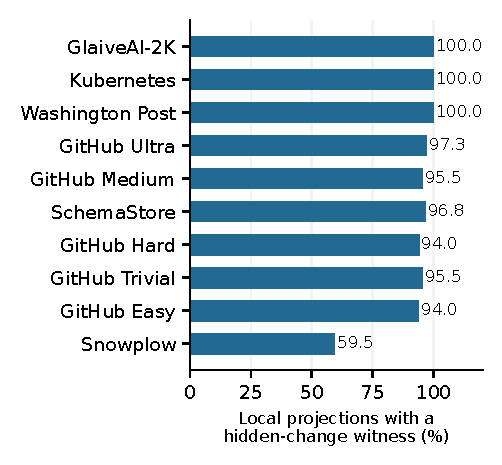
\includegraphics[width=\columnwidth]{figures/exposure.pdf}
\caption{Existence of a hidden-change witness in each local numeric projection, by corpus group. Percentages are conditional on the fixed stress palette. They measure neither full-schema reachability nor generation frequency.}
\label{fig:exposure}
\end{figure}

\begin{table}[t]
\centering\footnotesize\setlength{\tabcolsep}{3pt}\begin{tabular}{lrrr}
\toprule
Pipeline & Accepted & Changed & Rejected \\
\midrule
Native JS / MCP & 8,207 & 2,600 & 0 \\
Native Python & 7,990 & 479 & 217 \\
Post-parse integer check & 5,622 & 479 & 2,585 \\
Library number check & 5,242 & 0 & 2,965 \\
Raw-argument guard & 5,607 & 0 & 2,600 \\
Schema + argument guard & 5,543 & 0 & 2,664 \\
Lossless JSON & 8,207 & 0 & 0 \\
\bottomrule
\end{tabular}

\caption{Results on 8,207 distinct exact-valid pairs. ``Changed'' counts accepted outputs whose mathematical value differs from the source. SDK and native JavaScript outputs agree. Lossless wrappers require compatible downstream handling.}
\label{tab:results}
\end{table}

\subsection{Established remedies differ in availability}
Table~\ref{tab:results} shows that the post-parse integer check still admits 479 changed values, including decimal truncation and underflow to zero; 472 pass Ajv. Native Python also changes 479 accepted values while preserving ordinary arbitrary-precision integer tokens. Switching the language alone does not provide a universal fidelity guarantee.

The argument guard rejects exactly the 2,600 changing values and admits the 5,607 faithful ones. The joint guard rejects another 64 faithful arguments because their schemas contain changing numeric constraints. This is a conservative contract-level choice, not evidence that those individual arguments are erroneous. The existing library number check admits 5,242 values without changes; its safety predicate is more conservative than the measured wire-equality predicate. Lossless serialization preserves all 8,207 values and has the greatest transport availability in this test.

Four separate schema-collision fixtures use a rounded constant or bound and a faithful argument that is invalid under the exact source schema. Ajv and the argument-only guard admit all four; the joint guard rejects all four. These witnesses show why schema capture matters, but preserving schema bytes still does not guarantee exact validator arithmetic. For example, native division in a \texttt{multipleOf} check is a separate source of disagreement.

In the independent 15,265-token family, native transport changes 9,686 values. The guard has no false acceptances or false rejections relative to the rational wire oracle, and lossless serialization changes no value. This is bounded executable evidence for the implementation, not a proof about every possible JSON document.

\subsection{Wrong-record execution is observable end to end}
The native MCP handler returns the wrong fixture record for 25 of 54 requests and the correct record for 29 (Figure~\ref{fig:demo}). No request is rejected. Guarded ingress completes the same 29 faithful requests and rejects the other 25 before the handler. Under the explicit string identifier contract, all 54 requests select the intended record. These are deterministic fixture outcomes; no sampling uncertainty or model-accuracy inference is attached to them.

\begin{figure}[t]
\centering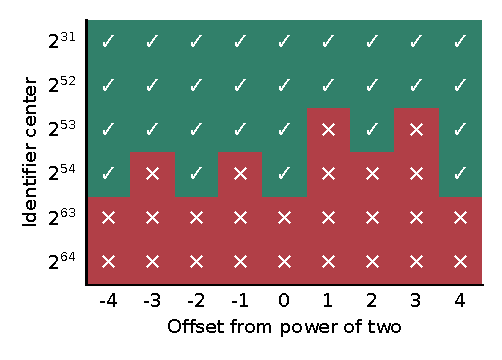
\includegraphics[width=\columnwidth]{figures/demo.pdf}
\caption{Native MCP lookup outcomes for constructed identifiers $2^e+d$. A cross indicates a wrong fixture record; a check indicates the requested record. Guarded ingress rejects each cross, while the string contract resolves every cell correctly.}
\label{fig:demo}
\end{figure}

\subsection{Runtime cost is measurable, not negligible}
We measure parse--serialize batches on shared macOS arm64 hardware with Node 24.19.0. For each input size and method, we run 100 warmups and nine batches of 500 iterations, rotating method order. Inputs contain ordinary faithful numbers; this benchmark measures the accepting path, excluding validation and network time. Figure~\ref{fig:timing} reports medians and observed batch ranges.

At 1,005 bytes, median native, guard, and lossless times are 14.2, 140.6, and 50.7 microseconds. At 67,701 bytes, they are 0.661, 6.915, and 2.557 milliseconds. The reference guard is slower than the existing lossless library in this workload. Shared-machine variability is large; these results neither establish deployment latency nor justify a negligible-overhead claim.

\begin{figure}[t]
\centering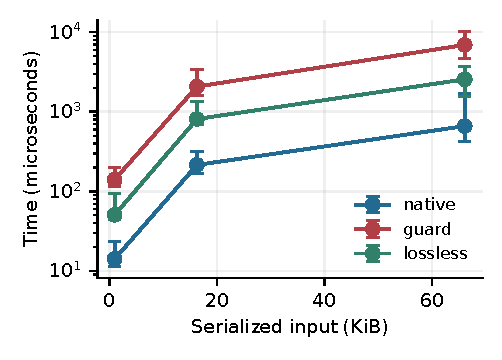
\includegraphics[width=\columnwidth]{figures/timing.pdf}
\caption{Local parse--serialize timing on faithful payloads. Points show medians of nine batches; bars show observed minimum and maximum batch means. Logarithmic vertical scale.}
\label{fig:timing}
\end{figure}

\section{Operational Implications}
Tool evaluation should preserve three observations: the raw emitted argument, the schema before its first numeric parse, and the value presented to the handler. A correct model output followed by a changing transport should be attributed to the transport. An incorrect emitted value should remain a model or prompting error. Post-parse logs alone cannot support this distinction.

For opaque record identifiers, an explicit string contract avoids accidental numeric interpretation and is supported by longstanding interoperability guidance. This is a schema migration: silently converting an existing numeric field to a string can violate the receiver's contract. For genuine exact numerical quantities, a lossless representation and compatible validation/application arithmetic are more appropriate. A refusal guard offers a narrower option when existing native-number components cannot be replaced, at a measurable availability cost.

A commercial integration could expose this audit as a schema registry check, a gateway preflight, or regression tests for SDK upgrades. Those are plausible product applications, not measured customer benefits or patentability claims. Exact monetary arithmetic, authorization, duplicate-key rejection, request limits, and transaction correctness require additional controls. A faithful decimal value does not by itself establish a safe financial operation.

\section{Conclusion}
Schema-valid tool arguments can change before execution, and downstream validation can accept the changed value. The pinned MCP reproduction demonstrates a wrong-record consequence; the public-schema audit identifies both broad local exposure and a much smaller set of existing drifting literals. Existing lossless transport and explicit string identifier contracts resolve the tested cases more completely than post-parse integer checking. The resulting evaluation protocol treats numeric wire fidelity as an independently testable property of LLM tool infrastructure.

\section*{Limitations}
The evidence comes from a public schema corpus, deterministic stress tests, and a local integration. There is no production deployment, measured user benefit, model-generation study, or estimate of incident frequency. Numeric projections omit enclosing and referenced constraints and cannot certify complete-schema satisfiability. Repeated definitions and related schemas are dependent; unique pairs and projection occurrences are reported separately. Corpus examples can be synthetic and do not establish genuine customer identifiers. The benchmark's known unsatisfiable schemas further restrict reachability claims.

The exact reference covers the retained numeric fragment, not all JSON Schema vocabularies, formats, reference resolution, or language-specific API semantics. Native validators can disagree even when every number is wire-faithful. The guard addresses numeric parse--serialize drift only, assumes duplicate-free JSON, and depends on reviver source support. Its prototype ingress shim is experimental and requires production hardening for framing, resource limits, and error handling. Lossless wrappers require compatible validators and arithmetic; normalizing them to native numbers can reintroduce the problem.

Results concern the pinned SDK, Ajv, library, Python, and Node versions; no vendor-wide or protocol-wide vulnerability claim follows. Runtime timings were collected on a shared machine, not a dedicated deployment benchmark. The simple collision proposition and guard predicate formalize established parsing principles. The claimed contribution is their schema-conditioned empirical evaluation and local tool reproduction, not a new number system or general parser-testing method. The literature search cannot establish absolute novelty.

\section*{Ethical Considerations}
The artifact uses public schemas and local fixture records. Wrong-record execution is demonstrated in an isolated process; no external service is mutated. Releasing bounded test cases helps maintainers reproduce transport behavior without treating ordinary numeric precision limits as evidence of malicious conduct. Logs of real tool traffic may contain confidential identifiers and content; deploying the proposed instrumentation would require appropriate retention and access controls.

\ifdefined\anonymous\else
\section*{Acknowledgments and Research Assistance}
Generative AI tools contributed to research ideation, literature discovery, code, mathematical exposition, experiment execution, figures, and manuscript drafting. The reported local experiments were executed; they are not model-generated numerical estimates. This manuscript requires substantive author verification and revision before submission. Automated checks do not constitute independent peer review.
\fi

\bibliography{references}
\bibliographystyle{acl_natbib}

\appendix
\section{Reproduction and Evidence Map}
The artifact includes source code, a pinned npm lockfile, Python package versions, corpus-file hashes, exact test inputs, raw transport outputs, local MCP requests/responses, and figure-generation code. The corpus revision is \texttt{9a94995b9279ae3a\allowbreak f3aed4b262917279\allowbreak 0b968d14}. Third-party corpus files can be downloaded by the supplied script; the reproduction verifies their hashes.

The primary run is:
\begin{quote}\scriptsize\ttfamily
npm ci\\
export NODE=node\\
C=../corpus/data\\
python3 scripts/build\_cases.py \$C\\
node scripts/run\_transport.mjs\\
node scripts/audit\_literals.mjs \$C\\
python3 scripts/analyze.py\\
python3 scripts/run\_demo.py\\
python3 scripts/property\_check.py\\
node scripts/schema\_witnesses.mjs\\
node scripts/benchmark.mjs\\
python3 scripts/figures.py
\end{quote}
Node 24 is recommended because the guard requires JSON reviver source context. The published measurements used Python 3.9.6, \texttt{jsonschema} 4.25.1, Matplotlib 3.9.4, and NumPy 1.26.4. Exact numeric results are deterministic; timing outputs will vary.

\paragraph{Audit records.}
\texttt{literal\_audit.json} records each changed literal with its file and JSON pointer. \texttt{summary.json} records distinct-pair and corpus-group counts. \texttt{transports.json} records every tested transformation and decision. \texttt{demo.json} stores full local protocol requests and responses. \texttt{property\_summary.json} and its inputs/outputs preserve the independent test family. Figure panels and table cells are generated from these files.

\section{Representative Witnesses}
\paragraph{Integer alias.}
With type integer, \texttt{9007199254740993} becomes \texttt{9007199254740992}; the result remains a valid integer.
\paragraph{Truncation and underflow.}
With type number, \texttt{0.10000000000000001} becomes \texttt{0.1}, while \texttt{1e-324} becomes zero. Both remain numeric.
\paragraph{Overflow.}
With type number, \texttt{1e309} serializes as null after native parsing. Strict finite-number validation rejects this case, so it is not a hidden-change witness.
\paragraph{Schema collision.}
An integer constant of \texttt{9007199254740993} and source argument \texttt{9007199254740992} collapse to the same native value. This source-invalid witness is evaluated separately from the exact-valid primary suite.


\paragraph{Guard normalization.}
For a decimal spelling with coefficient $c$ and exponent $e$, the normalizer computes $(c,e)$ using arbitrary-precision integers. It repeatedly divides nonzero $c$ by ten while incrementing $e$ until the coefficient is no longer divisible by ten. Equality of normalized pairs is equality of finite decimal rational values. This ignores insignificant spelling differences and signed zero. No rounding tolerance is used. The exact rational oracle is implemented separately in Python rather than sharing the guard's normalization code.

\paragraph{Duplicate keys and incomplete reachability.}
The excluded files are \texttt{Github\_hard/o84921.json} and \path{JsonSchemaStore/fossa-yml.v3.schema.json}. Excluding duplicate-key inputs avoids silently selecting a parser-specific first or last value. It does not solve full-schema reachability: even a duplicate-free full schema can be unsatisfiable, and a satisfiable schema may contain unreachable local numeric projections.

\paragraph{Guard scope.}
The schema-and-argument variant checks all numeric literals in each tested local projection. A production implementation could instead inspect only relevant schema assertions, resolve references, and retain provenance across each transformation. That extension is not evaluated here. A schema-fidelity guard must not be described as proving full validation correctness: exact divisibility and related arithmetic require their own reference semantics.
\end{document}
